\documentclass[12pt,a4paper]{article}
\usepackage[T1]{fontenc}
\usepackage{lmodern}
\usepackage[margin=2.5cm,headheight=15pt]{geometry}
\usepackage{amsmath,amssymb,amsthm,bm}
\usepackage{graphicx,booktabs,array}
\usepackage[numbers,sort&compress]{natbib}
\usepackage{fancyhdr}
\usepackage{microtype}
\usepackage{enumitem}
\usepackage{listings}
\usepackage[colorlinks=true,linkcolor=blue,citecolor=blue,urlcolor=blue]{hyperref}
\hypersetup{pdftitle={ETF Simulation with Temporal Memory: A Positive Fractional-Diffusive Volatility Model},pdfauthor={Enia Ardid and Pablo Casado de Amezu\'a}}
\pagestyle{fancy}\fancyhf{}
\fancyhead[L]{ETFs Simulation with Temporal Memory}
\fancyhead[R]{\thepage}
\renewcommand{\headrulewidth}{0pt}
\setlength{\parskip}{0.3em}
\setlength{\parindent}{0pt}
\setlength{\emergencystretch}{1em}
\linespread{1.06}
\newtheorem{proposition}{Proposition}
\newtheorem{remark}{Remark}
\newcommand{\E}{\mathbb E}
\newcommand{\R}{\mathbb R}
\newcommand{\one}{\mathbf 1}
\newcommand{\diag}{\operatorname{diag}}
\newcommand{\F}{\mathcal F}
\lstset{basicstyle=\ttfamily\footnotesize,breaklines=true,frame=single,columns=fullflexible}

\begin{document}
\hypersetup{pageanchor=false}
\begin{titlepage}
\begin{center}
\vspace*{0.5cm}
{\Large\bfseries ETFs Simulation with Temporal Memory:\\[0.25em]
A Positive Fractional--Diffusive Volatility Model\par}
\vspace{0.8cm}
{\large Enia Ardid, Pablo Casado de Amezu\'a\par}
\vspace{0.2cm}
{\small Research manuscript --- 19 October 2026\par}
\end{center}
\vspace{0.5cm}
\begin{abstract}
We study a positive conditional-variance model combining finite fractional-integral
memory and implicit diffusion on a correlation graph. We establish positivity,
fixed-parameter moment stability and exact multi-step variance forecasts for
the implemented recursion, without deriving it from an option-pricing equation.
A chronological study of the S\&P~500 and eleven sector ETFs uses 186 origins
during 2023--2026 and horizons of 1, 5 and 21 observations. Adding persistence,
asymmetry and multi-horizon validation improves the initial fractional model
in all six panel--horizon comparisons, but GJR-GARCH remains stronger. These
development results are exploratory. A further protocol fixes eight country
ETFs before download and retains the model unchanged. It adds FIGARCH and a
fixed 50:50 fractional/GJR forecast ensemble. The ensemble improves pooled QLIKE
over the standalone fractional model and FIGARCH in all nine comparisons
across the three panels. It exceeds GJR-GARCH in only three, with all paired
ranges against GJR including zero. The country panel does not confirm a
general diffusion benefit. The contribution is an explicit constrained
fractional--diffusive risk model and a reproducible assessment of its properties,
forecast combinations and limitations on retrospective adjusted-price data.
\end{abstract}
\vspace{0.3cm}
\textbf{Keywords:} fractional memory; conditional variance; graph diffusion;
sector ETFs; volatility forecasting; chronological validation.

\vspace{0.4cm}
\textbf{Data and code availability.} Code, tests, protocols and aggregate results
accompany this draft. The project repository is
\url{https://github.com/enia-ardid/mathematical_finance}.
The accompanying code and manuscript should be identified by their Git commit.
Raw prices are retained locally with source metadata and hashes and are not bundled.
\vfill
\begin{center}Research manuscript for author review; not a peer-reviewed publication.\end{center}
\end{titlepage}

\setcounter{page}{1}
\hypersetup{pageanchor=true}
{\small\setlength{\parskip}{0pt}\tableofcontents}
\clearpage

\section{Introduction}
Financial returns provide a difficult setting for directional forecasting:
recent prices already constitute a strong reference, while a visually plausible
price path can conceal weak predictive information. A more focused question is
whether temporal memory and sector interactions help forecast the magnitude of
future fluctuations. This paper retains those two ingredients and assigns them
to an explicit conditional-variance model.

Fractional filters provide flexible history weighting. Infinite fractional
differencing has a well-developed time-series interpretation
\citep{hosking1981}, and FIGARCH introduces hyperbolic persistence into conditional
heteroskedasticity \citep{baillie1996}. Neither construction implies that a Hurst
estimate can be inserted into an arbitrary stochastic recurrence. Likewise,
diffusion between economic categories requires a specified interaction operator;
an imposed ordering of sector names is not an observed spatial coordinate.
Graph operators offer an alternative for irregular domains \citep{shuman2013}.

Spatial ARCH models already allow conditional heteroskedasticity to depend on
neighboring locations \citep{otto2018}. For financial networks, network log-ARCH
models combine temporal effects with contemporaneous network interactions
\citep{mattera2024}. Our specification instead applies a positive graph
resolvent to lagged squared innovations with a shared finite fractional kernel.
It is a restricted multivariate ARCH model, rather than a new general class of
network volatility processes. The specific parameterization and its empirical
assessment must therefore be evaluated relative to that existing literature.

Our model applies a normalized finite fractional integral to squared standardized
innovations, then smooths this signal through a correlation-graph resolvent.
An explicit positive intercept and a feedback constraint control the resulting
variance recursion. This formulation differs from both a fractional
Black--Scholes equation and FIGARCH. It preserves the project's motivating idea
while making its actual stochastic object, initialization and mathematical
claims precise.

The contributions are threefold. First, we state and implement a positive
fractional--diffusive variance specification, with a graph construction that is
equivariant to relabeling assets. Second, we establish positivity, diffusion
contraction and fixed-parameter moment properties, and compute multi-step
conditional variances without simulation error. Third, we compare the method
against historical variance, tuned EWMA, GARCH and two structured ablations using
identical chronological forecast origins. These are contributions of formulation
and reproducible assessment; the study does not establish priority for the
general combination of fractional kernels and graph smoothing.

\subsection{Position relative to network volatility models}
Network GARCH already uses graph structure to reduce the dimension of
multivariate volatility estimation, with stationarity and QMLE results
\citep{zhou2020}. Threshold network GARCH also incorporates asymmetric shock
responses \citep{pan2024}. More recently, generalized network GARCH includes
neighboring shock and variance terms alongside covariance forecasts
\citep{zhou2026}. Neither network dependence nor asymmetry is original to the
present specification. Relative to these models, our restriction is a common
positive resolvent at every lag and a normalized fractional temporal profile.
Relative to FIGARCH, our finite normalized kernel and subunit feedback define
a different recursion; FIGARCH is fitted directly in the additional experiment
in Section~\ref{sec:external}. Published network models are discussed but not
fitted, so no comparative performance claim is made against them.

This narrower scope is intentional: an interpretable constrained model,
explicit assumptions, exact forecast moments and reproducible comparisons.
The mathematical results specialize positive-filter arguments rather than
claiming a new general stationarity theorem. The temporal/spatial restriction
is made explicit below through its impulse response.

The results support a narrower conclusion than universal predictive superiority.
The initial specification improves average losses relative to historical variance
and EWMA, but GARCH remains stronger. A persistent asymmetric refinement improves
all six pooled comparisons with that first specification and exceeds GARCH at
one and five observations in both US panels. GJR-GARCH remains stronger throughout
that standalone comparison. The additional external-universe study and fixed
forecast combination extend the assessment in Section~\ref{sec:external}.
Diffusion helps the one-session sector average modestly, with uncertainty ranges
including zero. Both the improvement and the stronger counterexample are needed
to assess the contribution of the fractional and diffusive components.

\section{Data, notation and prediction target}
\subsection{Observed prices and returns}
Let $P_{t,j}>0$ denote the closing price of asset $j$ at retained trading
observation $t$, and define
\begin{equation}
r_{t,j}=\log(P_{t,j}/P_{t-1,j}).
\label{eq:returns}
\end{equation}
The information available at forecast origin $o$ is
$\F_o=\sigma(P_0,\ldots,P_o)$. All transformations, graph estimates and parameter
choices used to forecast from $o$ depend only on this information.

The market snapshot was downloaded on 17 October 2026 from Yahoo Finance through
\texttt{yfinance} 0.2.66, with adjusted prices and an exclusive request end date
of 17 October 2026. It contains the index \texttt{\^{}GSPC} and the eleven ETFs
XLB, XLE, XLF, XLI, XLK, XLP, XLRE, XLU, XLV, XLY and XLC. After inception trimming
and alignment, common prices run from 19 June 2018 through 16 October 2026.
Prices must be positive, finite, uniquely dated and increasing in date; missing
interior observations are not filled.

The index and ETF panel are fitted separately. Adjusted ETF returns and an index
price-return series are not identical economic objects; we do not interpret
their combination as a self-financing index replication. The snapshot is
retrospective and may contain adjustment revisions unavailable at historical
forecast dates. Chronological code prevents access to future rows, but it does
not turn revised data into point-in-time observations.

\subsection{Risk target and common mean convention}
At each parameter refit, estimate a mean $\mu_j$ and a positive scale $s_j^2$
from the observed fitting window. These estimates are shared by all benchmark
models until the next refit. Write
\begin{equation}
u_{t,j}=r_{t,j}-\mu_j,\qquad z_{t,j}=u_{t,j}^2/s_j^2.
\end{equation}
The $h$-observation evaluation target is
\begin{equation}
Y_{o,h,j}=\sum_{\ell=1}^{h}(r_{o+\ell,j}-\mu_j)^2,
\qquad h\in\{1,5,21\}.
\label{eq:proxy}
\end{equation}
This is a daily squared-return proxy, not intraday realized variance. Under the
specified constant conditional mean it is conditionally unbiased for the sum of
future conditional variances. If the fitted mean differs from the true
conditional mean, the target also contains the corresponding squared mean
error. We therefore interpret the empirical task conservatively as forecasting
centered return second moments.

\section{A positive fractional--diffusive model}
\subsection{Finite fractional-integral memory}
For $0<d\le1$, the binomial expansion of $(1-B)^{-d}$ yields positive coefficients
\begin{equation}
g_0(d)=1,\qquad
g_k(d)=\frac{k-1+d}{k}\,g_{k-1}(d)
=\frac{\Gamma(k+d)}{\Gamma(d)\Gamma(k+1)}.
\label{eq:weights}
\end{equation}
With memory length $M$, normalize these coefficients:
\begin{equation}
p_k(d)=\frac{g_k(d)}{\sum_{v=0}^{M-1}g_v(d)},\quad
m_t=\sum_{k=0}^{M-1}p_k(d)z_{t-1-k}.
\label{eq:memory}
\end{equation}
Thus $p_k>0$ and $\sum_kp_k=1$. For large $k$, $g_k(d)$ behaves as
$k^{d-1}/\Gamma(d)$. Within a fixed window, increasing $d$ spreads weight toward
older observations; $d=1$ gives a uniform moving average. The study fixes
$M=252$. It does not infer $d$ from a Hurst estimator.

The normalized operator is a finite-window analogue of a fractional integral.
For a smooth signal $q$, a physical window $T$ and a refining observation step,
the corresponding normalized fractional integral is
\begin{equation}
\mathcal I_{d,T}q(t)=\frac{d}{T^d}\int_0^T a^{d-1}q(t-a)\,da.
\end{equation}
This relation motivates the kernel; the empirical model itself is the finite
discrete recursion \eqref{eq:memory}. Finite memory and subunit feedback do not
establish asymptotic long-range dependence or convergence to a fractional
stochastic PDE.

\subsection{Correlation graph and implicit diffusion}
Estimate a Ledoit--Wolf covariance matrix \citep{ledoit2004} after standardizing
the fitting-window returns. Convert it to a correlation matrix $R$ and set
\begin{equation}
W_{ij}=\max(R_{ij},0)^2\quad(i\ne j),\qquad W_{ii}=0.
\end{equation}
Let $D=\diag(W\one)$ and rescale the graph Laplacian by its mean degree:
\begin{equation}
L=\frac{D-W}{\max(J^{-1}\operatorname{tr}D,10^{-12})},\qquad
A_\tau=(I+\tau L)^{-1},\quad\tau\ge0.
\label{eq:diffusion}
\end{equation}
For the scalar index, $L=0$ and $A_\tau=1$; index results contain no evidence about
cross-sector diffusion. For sectors, the update $x=A_\tau m$ is the implicit
Euler step $x-m=-\tau Lx$ for graph heat diffusion. The diffusion parameter
controls smoothing on this estimated network, not a causal contagion rate.

No arbitrary one-dimensional sector ordering is required. Under a permutation
matrix $\Pi$, the same construction transforms $L$ into $\Pi L\Pi^{\mathsf T}$
and $A_\tau$ into $\Pi A_\tau\Pi^{\mathsf T}$. Forecasts are consequently
permutation equivariant.

\begin{figure}[tbp]
\centering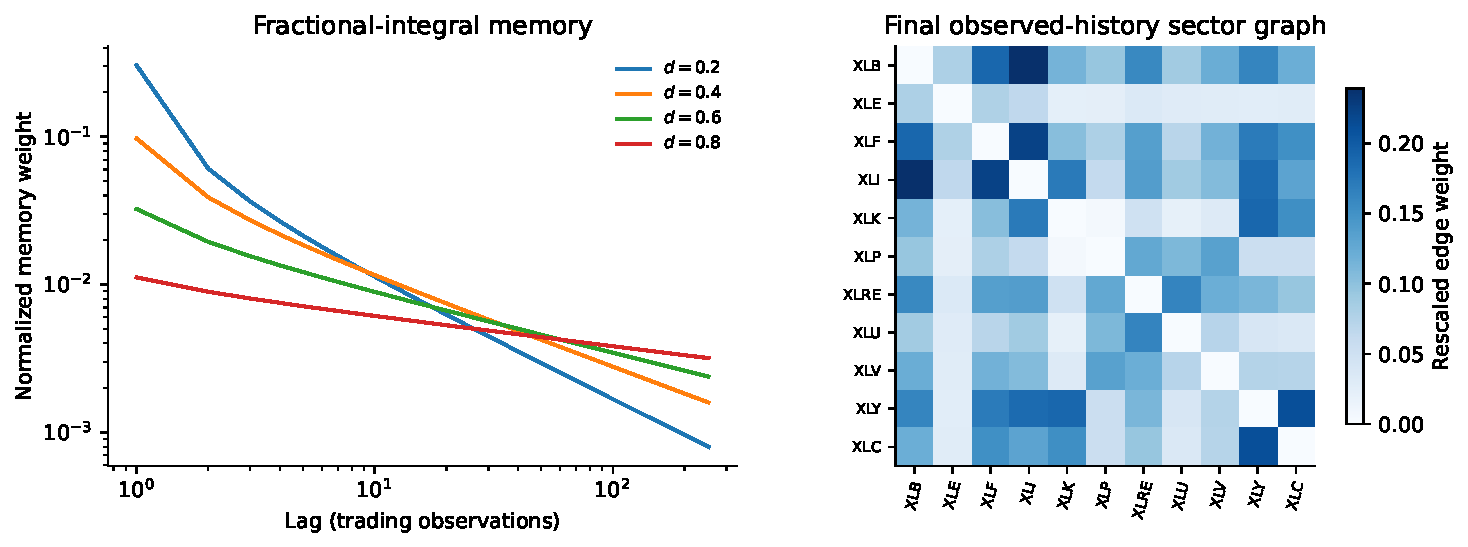
\includegraphics[width=\textwidth]{figures/kernel_graph.pdf}
\caption{Normalized fractional-integral weights and the sector graph from the
last parameter refit in the recorded backtest. The graph uses only the history
available at that refit. Weights are shown over the actual 252-observation
memory window; an infinite-memory interpretation is not assumed.}
\label{fig:kernel}
\end{figure}

\subsection{Conditional variance and return generation}
For $0\le\eta<1$, define normalized conditional variance $h_t$ and asset-scale
variance $v_t$ by
\begin{equation}
h_t=(1-\eta)\one+\eta A_\tau m_t,\qquad
v_t=s^2\odot h_t,
\label{eq:model}
\end{equation}
where $\odot$ denotes elementwise multiplication. Returns obey
\begin{equation}
r_t=\mu+\diag(\sqrt{v_t})\,\varepsilon_t,
\quad \E[\varepsilon_t\mid\F_{t-1}]=0,\quad
\E[\varepsilon_{t,j}^2\mid\F_{t-1}]=1.
\label{eq:returnmodel}
\end{equation}
For simulations, the implementation uses temporally independent Gaussian
innovation vectors with correlation $R$. Cross-sectional correlation does not
invalidate the marginal moment results below. Gaussian innovations are a
simulation assumption, not a claim that market return distributions are Gaussian.

Diffusion acts on standardized variance signals. It preserves their sum, not
necessarily the sum of variances in original asset units. This distinction
avoids forcing low-volatility and high-volatility sectors to have equal scale.
The positive intercept is explicit, and all simulated paths use the same stated
recursion rather than a fitted terminal price correction.

To make the connection with multivariate ARCH explicit, let
$S=\diag(s_1^2,\ldots,s_J^2)$. In asset units, the lag coefficient matrices are
$C_k=\eta p_k S A_\tau S^{-1}$, so that
$v_t=(1-\eta)s^2+\sum_{k=0}^{M-1}C_k(u_{t-1-k}\odot u_{t-1-k})$.
All $C_k$ are nonnegative, and
$\rho(\sum_k C_k)=\eta$. Fractional weighting and graph diffusion constrain
these matrices to an interpretable shared structure.

\clearpage
\section{Mathematical properties}
\begin{proposition}[Positive, nonamplifying graph diffusion]
For a symmetric nonnegative adjacency matrix and $\tau\ge0$, $A_\tau$ is
entrywise nonnegative and doubly stochastic. Its eigenvalues lie in $(0,1]$.
For any real vector $x$,
\begin{equation}
\min_jx_j\le(A_\tau x)_i\le\max_jx_j,\qquad
(A_\tau x)^{\mathsf T}L(A_\tau x)\le x^{\mathsf T}Lx.
\end{equation}
\end{proposition}
\begin{proof}
The Laplacian is symmetric positive semidefinite and $L\one=0$. Hence
$I+\tau L$ is invertible and $A_\tau\one=\one$. For $b\ge0$, a negative minimum
of the solution to $x+\tau Lx=b$ would make the corresponding left-hand component
negative, a contradiction. Thus $A_\tau\ge0$. Symmetry gives unit column sums.
The componentwise bound follows from convex averaging. Diagonalizing $L$ gives
eigenvalues $(1+\tau\lambda_i)^{-1}$ for $A_\tau$; the energy inequality follows
from $\lambda_i/(1+\tau\lambda_i)^2\le\lambda_i$.
\end{proof}

\begin{proposition}[Positivity and fixed-parameter moment stability]
Fix $M<\infty$, $s_j^2>0$ and $0\le\eta<1$. For nonnegative observed squared
innovations, $v_{t,j}\ge(1-\eta)s_j^2$. If the innovation vectors are iid over time
with zero means and unit marginal second moments, the normalized squared-return
recursion admits a unique causal stationary solution with finite first moments,
and its stationary marginal expectations satisfy $\E z_t=\one$. Consequently,
the corresponding stationary returns have variance $s_j^2$ and finite second
moments $\mu_j^2+s_j^2$.
\label{prop:stability}
\end{proposition}
\begin{proof}
The lower bound follows from nonnegative weights and nonnegative diffusion.
If initial component expectations are bounded by $C\ge1$, then
$\E h_{t,j}\le(1-\eta)+\eta C\le C$, and $\E z_{t,j}=\E h_{t,j}$.
For two histories driven by the same innovation sequence, put
$e_t=\E\lVert z_t-z_t'\rVert_1$. Independence of the current innovations from the
past, unit marginal second moments and the unit column sums of $A_\tau$ give
\begin{equation}
e_t\le\eta\sum_{k=0}^{M-1}p_ke_{t-1-k}.
\label{eq:coupling}
\end{equation}
The largest expected discrepancy contracts by at least $\eta$ each time an
entire block of $M$ initial lags is replaced. Backward iteration from a bounded
deterministic history is therefore Cauchy in $L^1$, yielding a causal stationary
limit; the same bound gives uniqueness among finite-first-moment solutions.
In stationarity, $b=\E z_t$ solves
$b=(1-\eta)\one+\eta A_\tau b$. Since $\rho(\eta A_\tau)<1$, its unique solution
is $b=\one$.
\end{proof}

These results concern fixed parameters. Rolling estimates need not form a
stationary process, and finite second moments do not imply finite fourth moments,
asymptotic normality of loss averages, or guaranteed forecast accuracy. The
finite-window contraction also explains why a power-shaped kernel should not
be advertised as a proof of infinite-horizon long memory.

\section{Forecasting and estimation}
\subsection{Exact multi-step marginal moments}
At origin $o$, let $\bar z_{o+\ell\mid o}$ equal observed $z$ for nonfuture lags,
and recursively replace future squared innovations by their conditional
expectations:
\begin{equation}
\bar h_{o+\ell\mid o}
=(1-\eta)\one+\eta A_\tau
\sum_{k=0}^{M-1}p_k\bar z_{o+\ell-1-k\mid o},\qquad
\bar z_{o+\ell\mid o}=\bar h_{o+\ell\mid o}.
\end{equation}
Linearity and unit innovation second moments make this recursion exact under
the fitted variance model. The aggregate forecast is
\begin{equation}
\widehat V_{o,h}=s^2\odot\sum_{\ell=1}^{h}\bar h_{o+\ell\mid o}.
\label{eq:aggregate}
\end{equation}
With the model's conditional mean, this also gives the marginal conditional
variance of cumulative future log-returns because the centered increments are
martingale differences. It does not provide an exact Gaussian predictive law
for their sum: future variances are themselves random. The study evaluates
variance forecasts directly and does not exponentiate an assumed Gaussian
multi-step law into a purported exact expected price.

\subsection{Chronological selection}
Forecast origins occur every five retained observations on a grid beginning at
price position 252; scoring begins in 2023. At the first scored origin and whenever
at least 21 observations have elapsed since the last refit, parameters are
updated. This gives a 25-observation refit spacing on the five-observation grid,
with 38 refits per panel in the reported experiment.

At a refit origin, reserve the final 252 observed returns for validation. Means,
scales and graph structure used to compute validation predictions are estimated
strictly before that block, using at most 1,008 returns. As validation advances,
already observed squared returns may update the memory state. Their future
counterparts are never accessed. Select the minimum pooled one-step QLIKE over
\begin{align}
d&\in\{0.2,0.4,0.6,0.8\}, &\eta&\in\{0.8,0.95,0.99\},\\
\tau&\in\{0,0.25,1,4\}.&&
\end{align}
The index fixes $\tau=0$. Stable candidate order resolves exact ties. After
selection, refit means, scales and the graph on the last 1,008 available returns,
including validation observations, and forecast subsequent targets. This is a
chronological selection design, not an untouched final test: the historical
period was available during earlier research iterations.

The same selected parameters serve all three horizons. Consequently, favorable
one-step validation does not guarantee optimal 21-step predictions. All methods
are scored at the same origins, excluding end blocks without complete targets
for every horizon.

\subsection{Benchmarks and ablations}
\begin{enumerate}[leftmargin=*,itemsep=0.2em]
\item \textbf{Historical variance:} the current fitting-window sample variance,
held constant over each forecast horizon.
\item \textbf{EWMA:} squared-innovation averaging with decay selected from
$\{0.9,0.94,0.97,0.99\}$ on the same validation block. Its future conditional
variance remains constant under its own update equation.
\item \textbf{GARCH(1,1):} independent asset models estimated by Gaussian
quasi-maximum likelihood \citep{bollerslev1986}. Positivity is imposed and
$\alpha+\beta<0.999$. Two fixed initializations are used; all 456 selected
asset-level fits report convergence in this run. No benchmark fit is replaced
silently by a weaker model.
\item \textbf{Fractional only:} the proposed kernel and feedback with $\tau=0$,
with its own validation-selected $d$ and $\eta$.
\item \textbf{Exponential plus graph:} replace the fractional average by EWMA
while retaining positive feedback and graph diffusion. Its decay, feedback and
diffusion grids have the same candidate count as the fractional graph model.
\end{enumerate}

The last two comparisons distinguish the contribution of graph smoothing from
the shape of the memory kernel. They are stronger checks than comparing only
against a constant price or historical variance.

\section{Evaluation of the initial specification}
\subsection{Loss and dependence}
The primary score is a normalized QLIKE loss,
\begin{equation}
\mathcal L_{o,h,j}=\log\left(\frac{\widehat V_{o,h,j}}{h s_j^2}\right)
+\frac{Y_{o,h,j}}{\widehat V_{o,h,j}}.
\label{eq:qlike}
\end{equation}
The normalization is known at the origin and common to all methods. It changes
the level, not paired comparisons. QLIKE is appropriate for conditional
second-moment forecasting with noisy, conditionally unbiased proxies
\citep{patton2011}; that robustness does not remove sampling noise or mean-model
error. Scores can be negative, and ratios of score levels are not reported as
percentage improvements. A normalized squared-error diagnostic is also retained
in the machine-readable results.

There are 186 common origins from 9 January 2023 to 17 September 2026, with
targets through 16 October 2026. The sector panel contributes 2,046 asset--origin
pairs per horizon, which must not be treated as independent replications.
Twenty-one-observation targets overlap. Paired circular block-bootstrap ranges
use 2,000 replicates, seed 1729, and blocks of five or ten origins. Entire sector
vectors are resampled together. These are nominal descriptive ranges; they do
not correct for all model selection, multiple comparisons, nonstationarity or
previous researcher exposure.

\subsection{Pooled comparison}
\begin{table}[tbp]
\centering\small\setlength{\tabcolsep}{4pt}
\begin{tabular}{lrrrrrr}
\toprule
 & \multicolumn{3}{c}{Index} & \multicolumn{3}{c}{Sectors} \\
Horizon & 1 & 5 & 21 & 1 & 5 & 21 \\
\midrule
Historical & 0.8368 & 0.6695 & 0.6737 & 0.8167 & 0.7187 & 0.7222 \\
EWMA & 0.8397 & 0.4576 & 0.5602 & 0.7195 & 0.5914 & 0.6251 \\
GARCH & \textbf{0.6004} & \textbf{0.3640} & \textbf{0.4714} & \textbf{0.6297} & \textbf{0.5499} & 0.6021 \\
Fractional only & 0.6514 & 0.4223 & 0.5467 & 0.6549 & 0.5638 & 0.6175 \\
Exponential + graph & 0.6690 & 0.3767 & 0.4841 & 0.6524 & 0.5542 & \textbf{0.5953} \\
Fractional + graph & 0.6514 & 0.4223 & 0.5467 & 0.6405 & 0.5627 & 0.6196 \\
\bottomrule
\end{tabular}

\caption{Mean normalized QLIKE at 1, 5 and 21 observations. Lower is better.
All methods use identical origins and the same mean convention. The index has
no cross-sector diffusion, so its two fractional rows coincide.}
\label{tab:main}
\end{table}

Table~\ref{tab:main} shows lower mean loss for fractional diffusion than tuned
EWMA at every panel--horizon combination. The one-session differences are
$-0.18834$ for the index and $-0.07899$ for sectors. Nevertheless, GARCH has lower
mean QLIKE in all six cases. For sectors, the proposed method's excess losses
relative to GARCH are 0.01084, 0.01287 and 0.01752 across the three horizons.
These findings support a useful alternative representation, not dominance over
standard conditional-variance models.

\begin{figure}[tbp]
\centering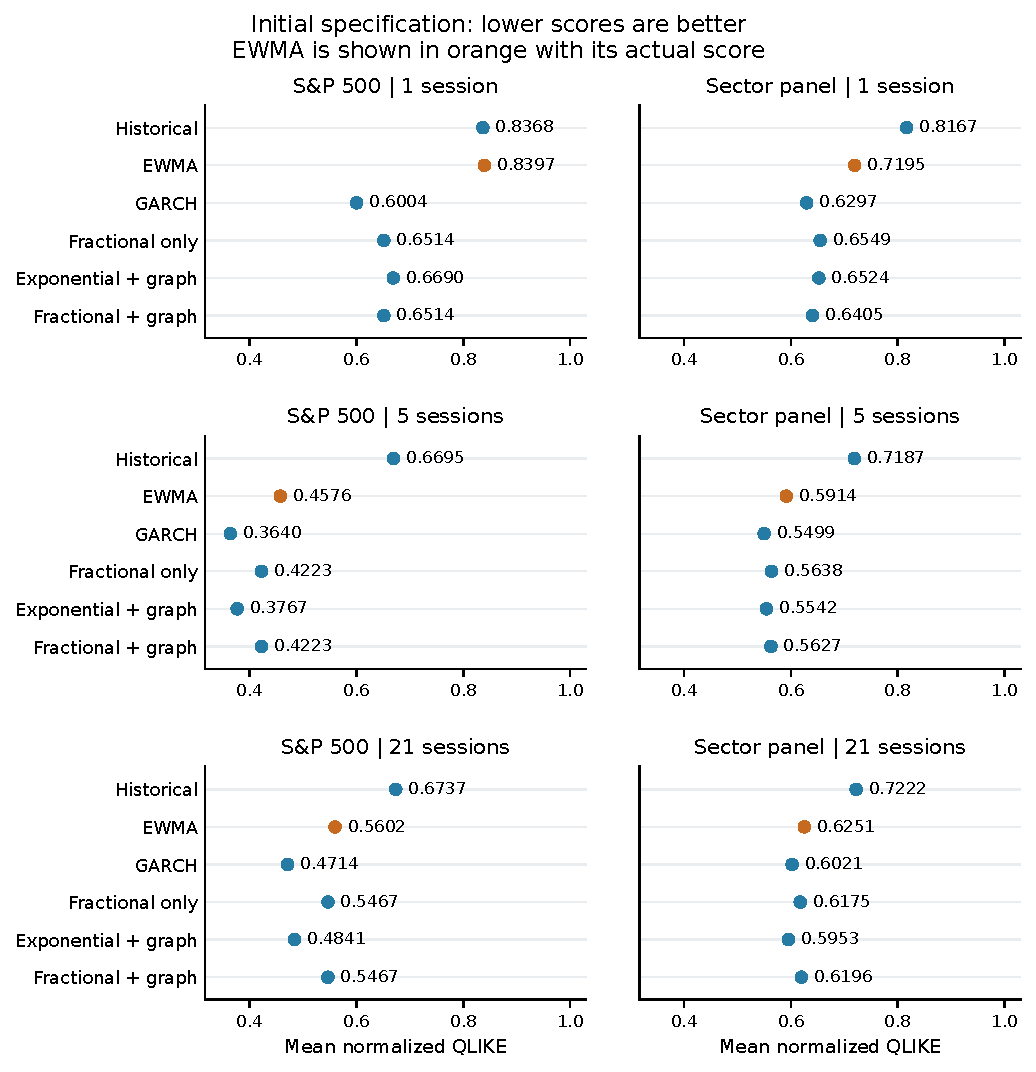
\includegraphics[width=\textwidth]{figures/forecast_comparison.pdf}
\caption{Mean normalized QLIKE for the initial specification and references.
Lower values indicate smaller loss. Each point and its numerical label show
the actual score, including EWMA in orange. The six panels share the same
horizontal scale and reproduce Table~\ref{tab:main}; all methods use identical
origins within each panel and horizon.}
\label{fig:comparison}
\end{figure}

Graph diffusion changes the one-session sector score from 0.65489 to 0.64053.
Its gain is much smaller at five observations, and the no-diffusion model is
slightly better at 21 observations. Nonzero diffusion is selected at 31 of 38
sector refits, but validation selection is not itself evidence of outer-sample
predictive benefit. The exponential graph model outperforms fractional diffusion
at five and 21 observations in both panels; the fractional kernel has the lower
one-session mean in both panels. Memory shape matters, but no shape dominates
all horizons.

With ten-origin blocks, the nominal 95\% range for the one-session sector
difference from EWMA is $[-0.26077,0.03470]$. Relative to no diffusion, it is
$[-0.03672,0.00145]$. Both include zero. The difference from GARCH is 0.01084,
with range $[-0.03822,0.04668]$. We therefore do not infer a reliable edge over
these dynamic references. Full ranges for both block lengths are distributed
with the generated tables.

\subsection{Variation over time}
\begin{figure}[tbp]
\centering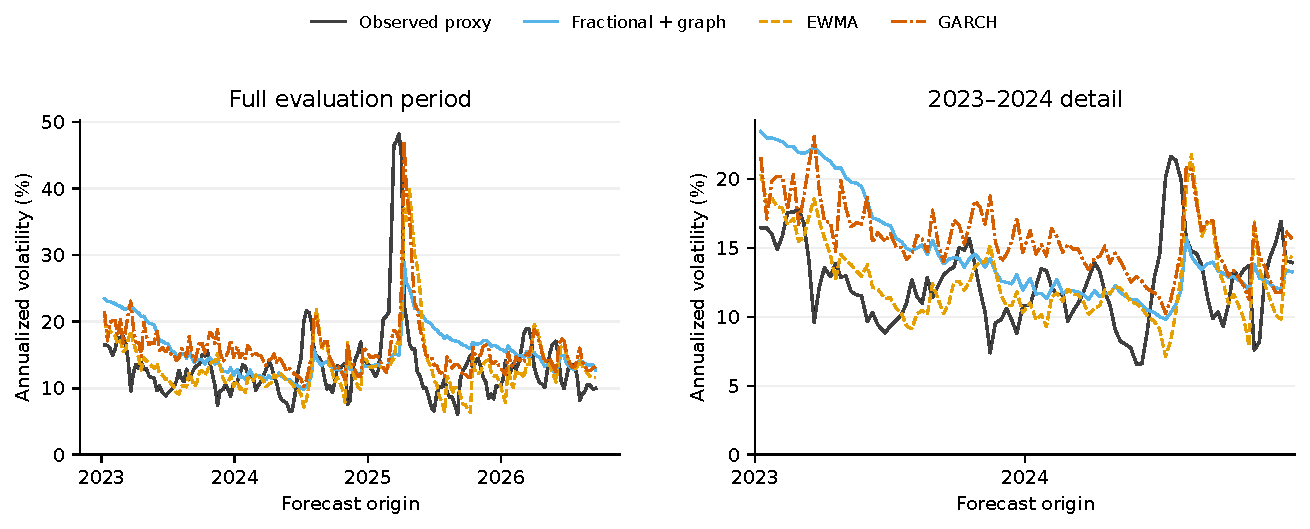
\includegraphics[width=\textwidth]{figures/variance_paths.pdf}
\caption{Index risk forecasts over 21 subsequent observations, displayed in
annualized volatility units. The gray series is the subsequently observed
squared-return proxy, plotted at its forecast origin for comparison; it was not
available then. The proxy is noisy and is not the latent conditional variance.}
\label{fig:paths}
\end{figure}

Average improvements are not uniform over calendar years. For the index, the
proposed method loses to EWMA at all horizons in 2023, wins at all horizons in
2024 and 2026, and has mixed results in 2025. For sectors, it loses at all
horizons in 2023 and improves on EWMA in the later years. The 2025 index
one-session difference of $-0.5367$ materially influences the pooled average;
it should not be interpreted as a stable gain in every regime.

Figure~\ref{fig:paths} illustrates the response to changing fluctuation levels.
The plot is descriptive and supplements the numerical losses; visual agreement
alone is not a forecast test. Annual scores and losses for every asset are
recoverable from the origin-level local outputs, while aggregate annual tables
are included in the manuscript bundle.

\section{Persistence and asymmetric innovations}
\label{sec:refinement}
\subsection{Specification and moment properties}
The initial model responds identically to positive and negative innovations and
selects parameters using only one-step losses. We retain its fractional kernel
and graph diffusion while allowing a persistent variance state and asymmetric
shock contributions. Define
\begin{align}
x_{t,j}&=z_{t,j}\frac{1+\delta\mathbf1\{u_{t,j}<0\}}{1+\delta/2},\\
h_t&=(1-b)(1-\eta)\one+b h_{t-1}
 +(1-b)\eta A_\tau\sum_{k=0}^{M-1}p_k x_{t-1-k},
\label{eq:refined}
\end{align}
with $v_t=s^2\odot h_t$, $0\le b<1$ and $\delta\ge0$. The parameter $b$
smooths the variance response. With $\delta=1$, a negative innovation has twice
the contribution of a positive innovation of the same magnitude.

For the asymmetric recursion, assume conditionally symmetric innovations with
unit second moments. This is stronger than a zero-mean, unit-variance assumption:
symmetry gives $\E[\varepsilon_{t,j}^2\mathbf1\{\varepsilon_{t,j}<0\}]=1/2$
and therefore $\E[x_t\mid\F_{t-1}]=h_t$. Gaussian simulation innovations satisfy
the assumption; it is not asserted as an empirical property of market shocks.
Future expected variances are obtained by the same substitution as in
Section~5.1, retaining the additional state $h_{t-1}$.

Unit initial variance and unit presample transformed squares give the floor
$v_{t,j}\ge(1-\eta)s_j^2$ by induction. For fixed parameters and iid symmetric
innovations, the shared-noise argument for Proposition~\ref{prop:stability}
now gives, for discrepancies between normalized variance processes,
\begin{equation}
e_t\le b e_{t-1}+(1-b)\eta\sum_{k=0}^{M-1}p_k e_{t-1-k},\qquad
b+(1-b)\eta<1.
\end{equation}
The maximum expected discrepancy over the finite lag state contracts over
successive $M$-observation blocks. The same backward-iteration argument yields
a unique causal finite-first-moment stationary variance process. Its mean is
$\one$, so return variance is $s_j^2$. The recursive state adds exponentially
decaying persistence; it does not establish asymptotic long-range dependence.

\subsection{Effective memory and graph modes}
The persistence state has an exact filter interpretation. For fixed parameters,
unroll \eqref{eq:refined} after removing its initialization transient to obtain
\begin{align}
h_t&=(1-\eta)\one+\eta A_\tau\sum_{j=1}^{\infty}\widetilde p_jx_{t-j},\\
\widetilde p_j&=(1-b)\sum_{k=0}^{\min(M-1,j-1)}p_k b^{j-1-k}.
\label{eq:effectivekernel}
\end{align}
Indeed, repeated substitution expands the state into a geometric sum; grouping
terms with the same innovation lag yields \eqref{eq:effectivekernel}. Since
all terms are nonnegative, summing in either order gives
$\sum_{j\ge1}\widetilde p_j=(1-b)\sum_kp_k\sum_{\ell\ge0}b^\ell=1$.
For $0<b<1$ and $j\ge M$, $\widetilde p_{j+1}=b\widetilde p_j$.
At $b=0$ the weights reduce to $p_{j-1}$ for $1\le j\le M$, with zero tail.
Thus the refinement geometrically smooths the finite fractional kernel; its
infinite tail, when present, is exponential rather than hyperbolic.

With $L=U\Lambda U^{\mathsf T}$, the graph-mode coefficient at lag $j$ is
$\eta\widetilde p_j/(1+\tau\lambda_\ell)$. Temporal weighting and spatial
smoothing are separable: every lag shares the same graph attenuation. This
clarifies both interpretability and a restriction relative to more general
network lag matrices. A numerical impulse-response test verifies the identity
against the implemented filtering recursion.

\subsection{Recorded follow-up protocol}
This refinement was designed after inspecting the initial study. The separate
\path{paper/refinement_protocol.json} records its rules before its candidates
were evaluated, but the historical targets are reused and no independent
confirmation is claimed. At each refit, use the same 252-observation validation
block and fit nuisance parameters strictly before it. Retain only validation
origins whose complete 21-observation targets finish by the refit date. Minimize
the equal-weight mean of normalized QLIKE at horizons 1, 5 and 21, using all
eligible daily origins. A single selected specification serves all outer horizons.

Retain the earlier grids for $d$, $\eta$ and $\tau$, and add
$b\in\{0,0.5,0.9\}$ and $\delta\in\{0,1\}$. There are 288 candidates for
sectors and 72 for the scalar index per kernel family. A symmetric variant fixes
$\delta=0$; a graph ablation fixes $\tau=0$; a kernel ablation uses normalized
exponential weights truncated to the same 252 observations, with the earlier
four decay values. Each ablation has its own validation selection. The larger
candidate set increases selection risk despite chronological ordering.

An additional GJR-GARCH reference permits asymmetric shock responses
\citep{glosten1993}. Its normalized variance satisfies
$h_t=\omega+(\alpha+\gamma\mathbf1\{u_{t-1}<0\})z_{t-1}+\beta h_{t-1}$.
Independent asset fits use Gaussian QMLE, two fixed starts, nonnegative
coefficients and $\alpha+\beta+\gamma/2<0.999$. All 456 selected fits report
convergence. Multi-step moments also require conditional symmetry. Earlier
reference forecasts are recomputed; all 40,176 original forecast records and
loss values match exactly, so comparisons use unchanged targets and scales.

\subsection{Follow-up results}
\begin{table}[tbp]
\centering\small\setlength{\tabcolsep}{4pt}
\begin{tabular}{lrrrrrr}
\toprule
 & \multicolumn{3}{c}{Index} & \multicolumn{3}{c}{Sectors} \\
Horizon & 1 & 5 & 21 & 1 & 5 & 21 \\
\midrule
Fractional + graph & 0.6514 & 0.4223 & 0.5467 & 0.6405 & 0.5627 & 0.6196 \\
Persistent symmetric & 0.6143 & 0.3815 & 0.5162 & 0.6447 & 0.5582 & 0.6116 \\
Refined fractional & 0.5819 & 0.3574 & 0.4977 & 0.6242 & 0.5478 & 0.6043 \\
Asymmetric, no graph & 0.5819 & 0.3574 & 0.4977 & 0.6317 & 0.5474 & 0.6046 \\
Asymmetric exponential & 0.6223 & 0.3516 & 0.4785 & 0.6656 & 0.5588 & 0.5980 \\
GARCH & 0.6004 & 0.3640 & 0.4714 & 0.6297 & 0.5499 & 0.6021 \\
GJR-GARCH & \textbf{0.5251} & \textbf{0.3128} & \textbf{0.4360} & \textbf{0.6053} & \textbf{0.5401} & \textbf{0.5931} \\
\bottomrule
\end{tabular}

\caption{Mean normalized QLIKE for the refinement, its ablations and references.
``Original fractional'' denotes the initial variance specification. All rows
use the same 186 origins. Lower is better.}
\label{tab:refinement}
\end{table}

Table~\ref{tab:refinement} shows lower pooled loss for persistent asymmetric
fractional diffusion than the initial model in all six comparisons. Index
scores change from $(0.65138,0.42225,0.54672)$ to
$(0.58187,0.35738,0.49770)$, and sector scores from
$(0.64053,0.56274,0.61963)$ to $(0.62417,0.54779,0.60432)$.
The refinement also has lower loss than GARCH at one and five observations in
both panels. GARCH remains better at 21 observations, while GJR-GARCH is better
at every panel--horizon combination. These findings establish improvement within
the studied fractional family without establishing dominance over asymmetric
volatility references.

\begin{figure}[tbp]
\centering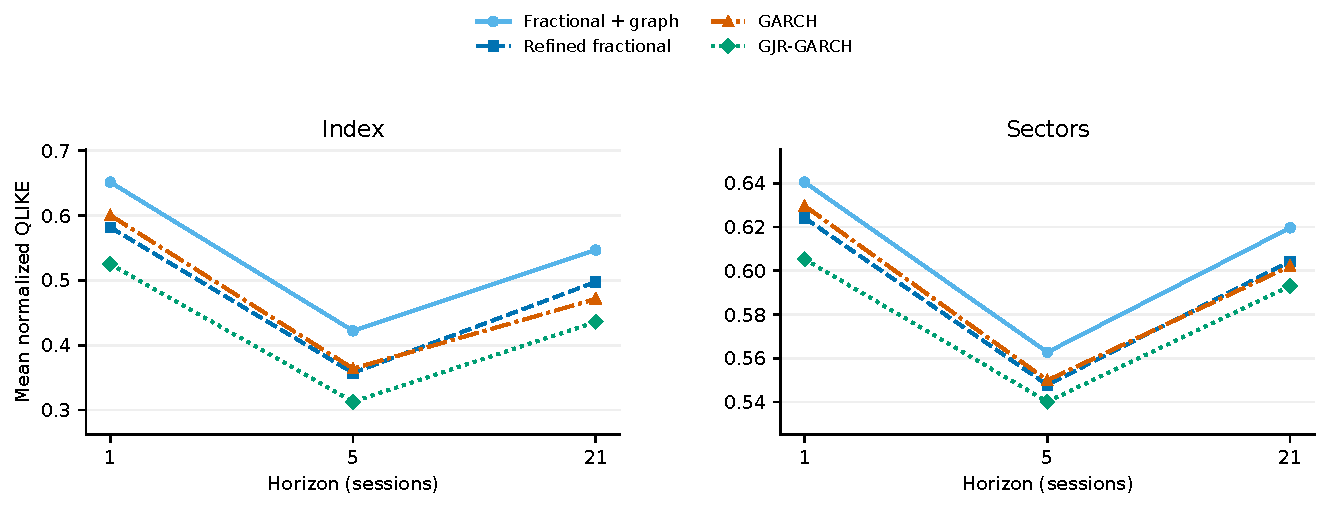
\includegraphics[width=\textwidth]{figures/refinement_comparison.pdf}
\caption{Pooled losses before and after the refinement, alongside GARCH and
GJR-GARCH. The asymmetric reference remains stronger in every displayed case.}
\end{figure}

Using ten-origin blocks, nominal 95\% ranges for the change relative to the
initial fractional model exclude zero in five of six comparisons; the exception
is one-session sector forecasting. For the index, the one-session change is
$-0.06952$ with range $[-0.14531,-0.00876]$. All ranges comparing the refinement
with GARCH include zero. These descriptive ranges do not adjust for the repeated
research on this snapshot and should not be read as independent confirmation.

Asymmetry is selected at all 38 index refits and 35 sector refits; nonzero
variance persistence is selected at every refit. The graph is selected with
nonzero strength at 18 sector refits. Relative to its graph ablation, the
refinement improves the one-session sector mean by 0.00752, slightly worsens the
five-session mean and changes the 21-session mean little. The exponential
ablation is stronger for index horizons 5 and 21 and sector horizon 21. Thus
neither graph smoothing nor the fractional kernel uniformly dominates its
alternative. Annual improvements also vary: relative to the first specification,
index loss rises at 21 sessions in 2024, and sector loss rises at 5/21 sessions
in 2024 and at one session in 2025. All annual results remain in the public tables.

\section{External-universe replication and a fixed forecast combination}
\label{sec:external}
\subsection{A specification fixed before the new download}
The previous two studies reuse US history inspected during development. To
assess transfer to another universe, a third protocol fixed eight country ETFs
before downloading their prices: EWA (Australia), EWC (Canada), EWG (Germany),
EWH (Hong Kong), EWJ (Japan), EWL (Switzerland), EWQ (France) and EWU (United
Kingdom). These are long-established US-listed iShares equity funds, selected
for geographical spread. The request covers 1 January 2018 through 16 October
2026, using the same adjusted-price convention. All eight assets are required;
missing prices are not filled and assets are not removed after seeing results.

The unchanged fractional implementation, parameter grids, validation windows,
refit schedule and three horizons are frozen in
\path{paper/external_protocol.json}, with source hashes. No external loss is
used to revise that specification. This is a locally timestamped protocol,
not an independently registered preregistration. The country panel was not
previously evaluated in this project, but it shares global shocks, US trading
hours and dollar denomination with the development assets. It is therefore an
external-universe replication on retrospective data, not a statistically
independent sample or a prospective experiment.

A computational amendment is recorded in the accompanying protocol files.
The first attempt reached the
FIGARCH forecast and failed because a strided panel column was not C-contiguous.
The correction copies input arrays to the required layout. It changes no
model or evaluation rule; no FIGARCH comparison results existed at that point.
The original protocol and failed-run record are retained.

\subsection{Additional forecaster and fractional benchmark}
The additional forecaster is deliberately fixed:
\begin{equation}
\widehat V^{\mathrm{ens}}_{o,h,j}
=\tfrac12\widehat V^{\mathrm{frac}}_{o,h,j}
+\tfrac12\widehat V^{\mathrm{GJR}}_{o,h,j}.
\label{eq:ensemble}
\end{equation}
Here the fractional component is the persistent asymmetric model, including
its selected graph diffusion. The coefficient is always one half, with no
fitted or retrospectively selected combination weights. Positivity is
preserved. The ensemble is an optional forecast combination, not a new
generative fractional recurrence, and does not replace the standalone model.
Its QLIKE is computed from the combined variance; component losses are not
averaged. Forecast combinations are not themselves a novelty claim.

FIGARCH(1,$d$,1) \citep{baillie1996} is added as an estimated benchmark using
\texttt{arch} 7.2.0, Gaussian QMLE and the library's 1,000-lag ARCH
approximation. Each asset is centered and standardized using the same
origin-fitted mean and scale as the other methods. Fit on the preceding
1,008 returns at the same refit dates, with default starting estimates and
SLSQP limited to 1,000 iterations. Between refits, keep parameters and the
fitting backcast fixed while updating on observed returns. Analytic forecasts
are transformed back to asset units and summed over the same horizons.
Nonfinite results abort the experiment; finite nonconverged fits are reported
rather than silently replaced. FIGARCH's approximation and initialization
differ from our normalized 252-lag kernel and are recorded explicitly.

The same ensemble and FIGARCH reference are appended to the recorded US
forecasts after checking their code and input hashes. Those comparisons remain
exploratory. Every table uses identical targets within its panel; pooled,
annual and asset-level losses are retained. Paired uncertainty ranges use the
same whole-panel circular bootstrap and the same nominal interpretation as
the earlier study.

\subsection{Results}
The international panel contains 2,210 prices per asset. Evaluation has
186 origins from 6 January 2023 to 16 September 2026, with complete targets
through 15 October 2026 and 38 parameter refits. Its five-observation grid
has a different calendar phase from the US grid; comparisons are paired
within panels. All 760 FIGARCH asset fits across the three panels converge,
as do all 304 international GARCH and 304 GJR-GARCH fits.

The unchanged fractional model obtains international QLIKE
$(0.52898,0.66359,0.67147)$ at horizons $(1,5,21)$, below both EWMA and FIGARCH
at every horizon. However, GARCH and GJR-GARCH are stronger at all three.
The no-graph ablation has lower loss throughout, while the exponential kernel
is better at horizons 5 and 21. Thus the second universe does not support a
general benefit from diffusion or a uniform fractional-kernel advantage.

The fixed ensemble lowers those fractional scores to
$(0.51307,0.65094,0.66134)$, improving all three external pooled comparisons.
Its asset-level loss is lower in 22 of 24 country--horizon comparisons, but
annual pooled loss worsens relative to the standalone fractional model at
horizons 5 and 21 in 2024. Across the US and international panels, the ensemble
improves on both the standalone fractional model and FIGARCH in all nine
panel--horizon comparisons. These are loss differences, not percentages of an
arbitrarily normalized score.

Relative to GJR-GARCH, the ensemble wins only for US sectors at 5 and 21
observations and for the international panel at 21 observations. The
international 21-session difference is $-0.00092$, with ten-origin-block
nominal 95\% range $[-0.01174,0.01110]$. All nine ensemble-versus-GJR ranges
include zero. For international one-session forecasts, the change from the
standalone fractional model is $-0.01590$; the interval is
$[-0.03100,-0.00219]$.

Compared with FIGARCH, the difference is $-0.03073$. Its interval runs from
$-0.05536$ to $-0.01145$. These descriptive intervals support reporting the
observed improvement without claiming reliable superiority over GJR-GARCH.
Full annual, asset-level and paired comparisons remain in the public outputs.


\begin{table}[tbp]
\centering\small
\begin{tabular}{lrrr}
\toprule
horizon & 1 & 5 & 21 \\
\midrule
EWMA & 0.5321 & 0.6700 & 0.6823 \\
GARCH & 0.5287 & 0.6587 & 0.6672 \\
GJR-GARCH & 0.5083 & 0.6496 & 0.6623 \\
FIGARCH & 0.5438 & 0.6671 & 0.6730 \\
Fractional & 0.5290 & 0.6636 & 0.6715 \\
Without graph & 0.5234 & 0.6633 & 0.6701 \\
Exponential kernel & 0.5290 & 0.6526 & 0.6653 \\
Fixed 50:50 ensemble & 0.5131 & 0.6509 & 0.6613 \\
\bottomrule
\end{tabular}

\caption{Mean normalized QLIKE on the eight pre-specified country ETFs.
The fractional row is the unchanged persistent asymmetric model. The fixed
ensemble averages its variance forecasts with GJR-GARCH. Lower is better.}
\label{tab:external}
\end{table}

\begin{figure}[tbp]
\centering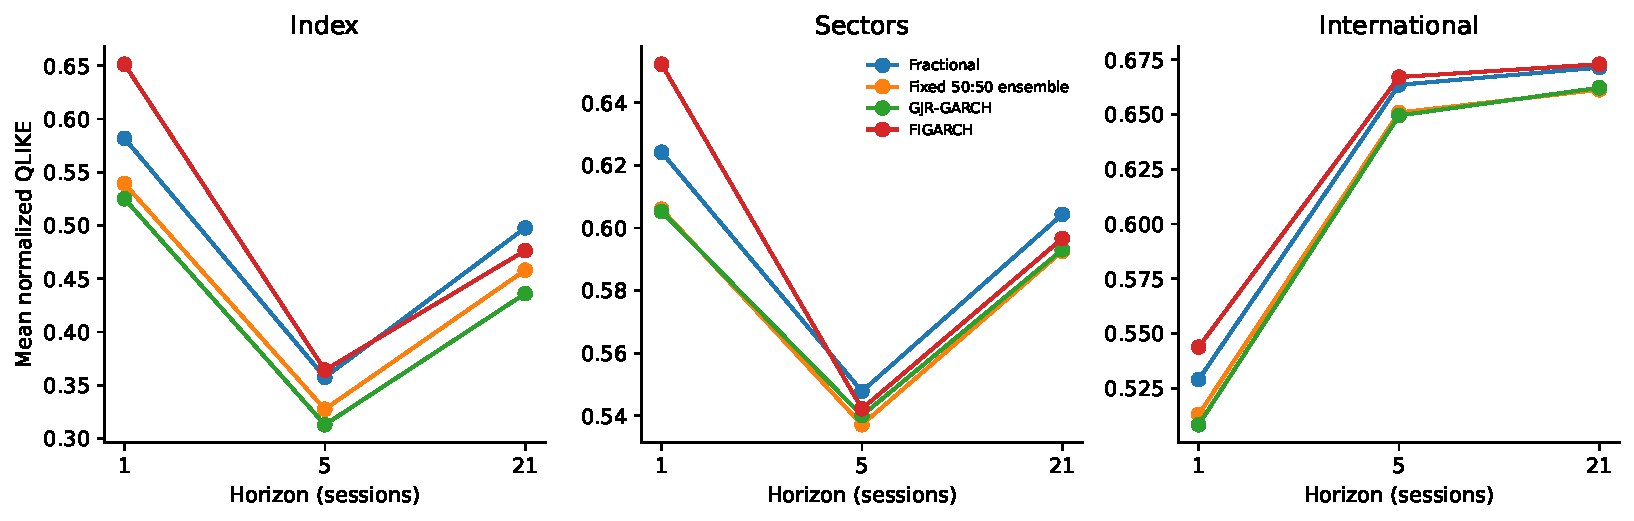
\includegraphics[width=\textwidth]{figures/external_comparison.pdf}
\caption{Standalone fractional forecasts, the fixed ensemble, GJR-GARCH and
FIGARCH. The index and sector panels reuse the development snapshot; the
international panel follows the separately recorded external-universe protocol.}
\label{fig:external}
\end{figure}

\subsection{Observed evolution and rolling predictions}
Aggregate losses summarize accuracy but do not show how forecasts respond over
time. Figures~\ref{fig:index-predictions} and~\ref{fig:panel-predictions} compare
the recorded predictions with the subsequently observed squared-return targets
over the full evaluation period. For readability, both are expressed in
annualized volatility units:
\begin{equation}
\widehat\sigma^{\mathrm{ann}}_{o,h,j}
=100\sqrt{\frac{252}{h}\widehat V_{o,h,j}},\qquad
\sigma^{\mathrm{proxy}}_{o,h,j}
=100\sqrt{\frac{252}{h}Y_{o,h,j}}.
\label{eq:display-volatility}
\end{equation}
These are square-root transformations of variance forecasts and noisy targets,
not estimates of an observed latent volatility path. In particular, the square
root of expected variance is not generally expected volatility. At one session,
the observed series is a scaled absolute centered return and is especially noisy.

The new time-series panels use the \emph{end of the target window} on the
horizontal axis. A prediction plotted at $o+h$ was issued at $o$, using only
the data available then. Curves join the retained origins, spaced five observed
sessions apart; they are not a new forecast issued every day. No further fitting,
time smoothing, clipping of peaks or favorable subperiod selection is applied.
The 21-session target windows overlap.

\begin{figure}[p]
\centering
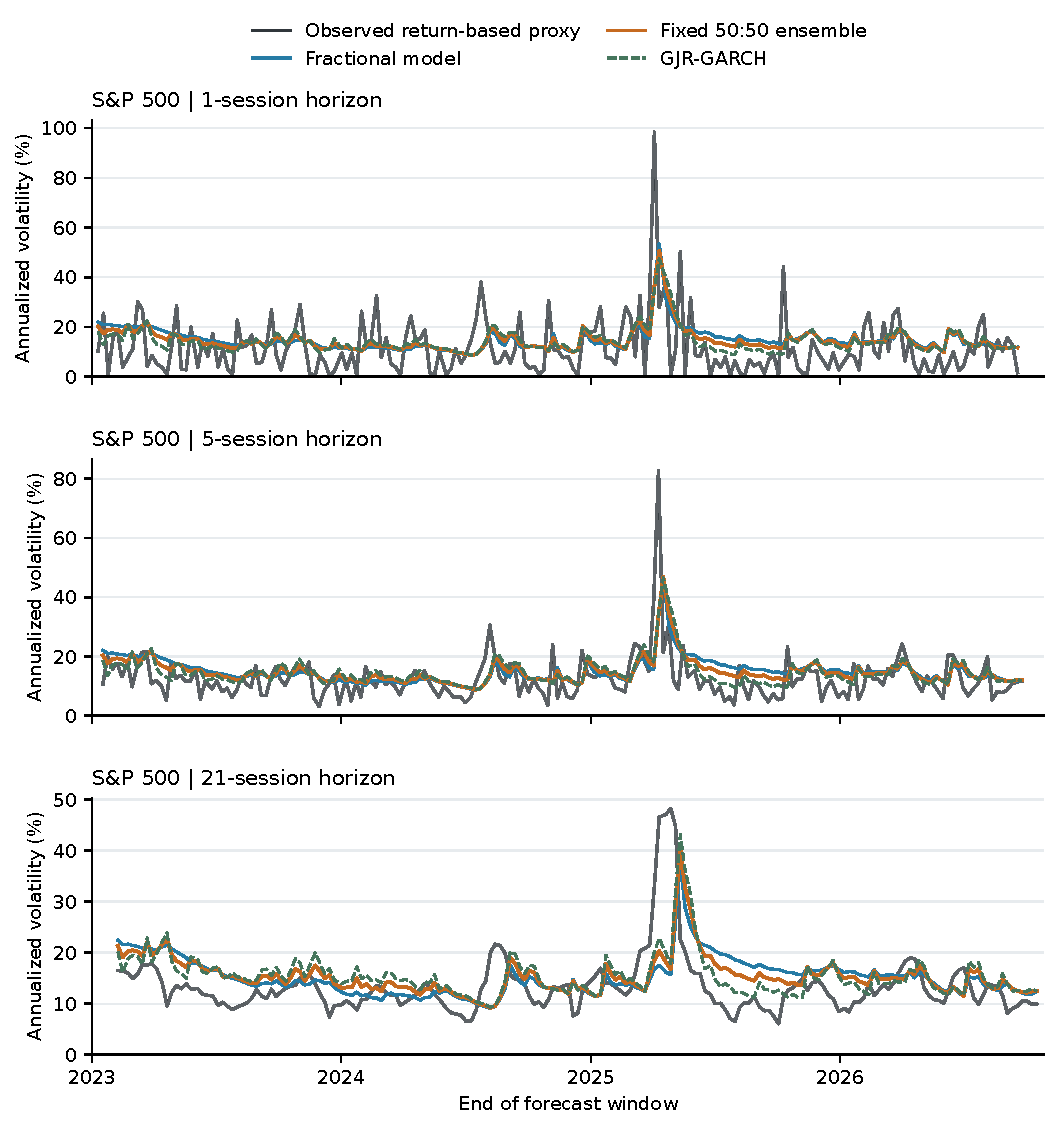
\includegraphics[width=\textwidth,height=.76\textheight,keepaspectratio]{figures/prediction_index_horizons.pdf}
\caption{S\&P~500 observed proxy and rolling predictions at 1, 5 and 21 sessions.
Black denotes the subsequent return-based observation; blue is the persistent
fractional model, orange the fixed ensemble, and dashed green GJR-GARCH. Each
forecast was issued the stated number of observations before its plotted
window-end date. Vertical scales differ by horizon to retain the full peaks.}
\label{fig:index-predictions}
\end{figure}

\begin{figure}[p]
\centering
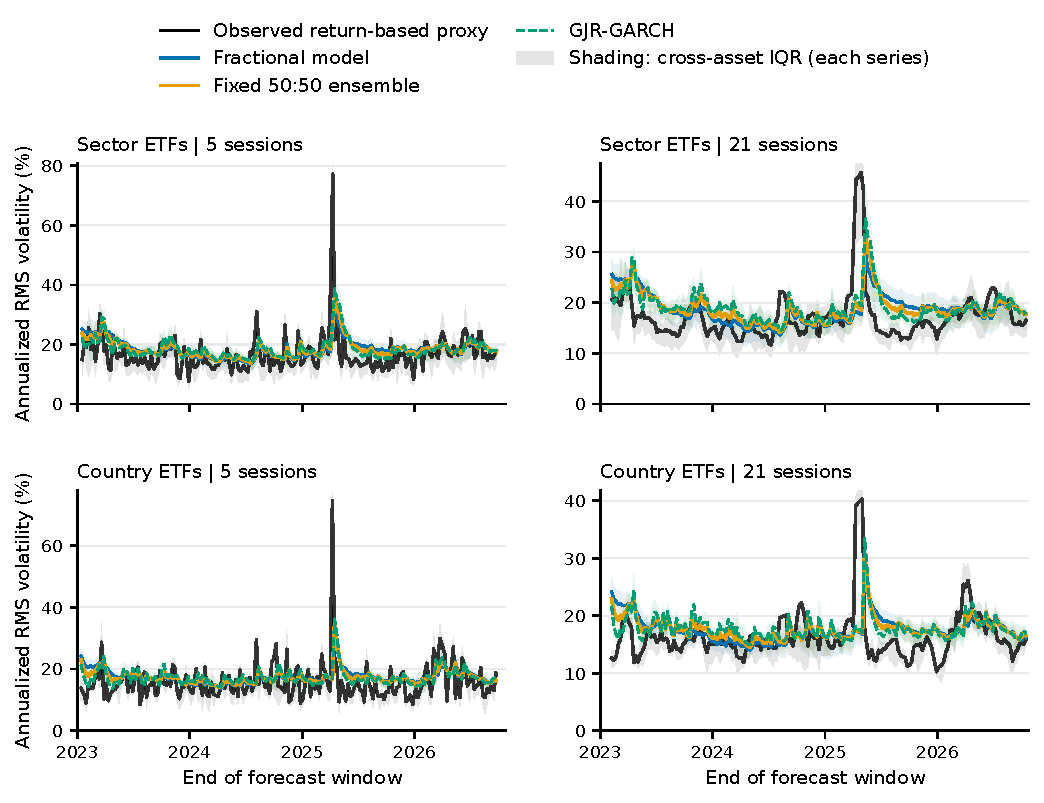
\includegraphics[width=\textwidth]{figures/prediction_panel_evolution.pdf}
\caption{Observed and predicted risk evolution for all eleven sector ETFs and
all eight country ETFs, at horizons of 5 and 21 sessions. Marginal variances
are averaged across the complete panel before taking the square root. These
are annualized root-mean-square marginal volatilities, not portfolio volatility;
cross-asset covariances are not included in this display.}
\label{fig:panel-predictions}
\end{figure}

For the multi-asset displays, average $\widehat V_{o,h,j}$ and $Y_{o,h,j}$ over
all assets before applying \eqref{eq:display-volatility}. Averaging volatilities
directly would give a different quantity. The panel curves can also mask
opposing asset-level errors. Appendix~\ref{app:asset-paths} therefore retains
the complete set of 21-session paths for every sector and country ETF. These
visual diagnostics complement the common-target losses and paired comparisons;
visual tracking alone does not establish predictive superiority.

The index curves also reveal limitations hidden by pooled scores. The abrupt
2025 increase is incompletely anticipated, and the persistent forecasts can
remain elevated after the observed proxy falls. Smoother predictions should
not be interpreted as pointwise reproduction of the realized fluctuations.

\clearpage
\section{Interpretation, limitations and conclusions}
The revised model preserves temporal fractional weighting and sector diffusion
while assigning both to a well-defined positive variance process. The graph
step is stable for every nonnegative diffusion strength, and the fixed-parameter
recursion has a finite-second-moment return interpretation. These are meaningful
improvements in mathematical specification. They do not repair the original
price-PDE derivation by assertion: the present model is a new variance
specification, and the earlier simulator is retained separately for continuity.

The empirical conclusions are limited by four features of the study. First,
the development and international panels use retrospective adjusted prices
and share market shocks; neither is a prospective evaluation. Second, daily
squared returns are noisy risk proxies. Third, the finite memory window,
parameter grids and constant conditional mean restrict the model. Fourth,
GJR-GARCH and several kernel-ablation comparisons remain stronger,
while descriptive uncertainty ranges often include zero.
FIGARCH is now fitted directly, but published network log-ARCH and network
GARCH specifications are not; no advantage over those families is established.

Further work should retain point-in-time inputs and evaluate genuinely future
targets, with richer volatility proxies and direct network-model benchmarks.
Graph estimation uncertainty, richer conditional innovation laws and
horizon-specific calibration remain open extensions. Claiming a causal contagion mechanism, a universally
superior forecaster, profitable trading, or an infinite-memory limit would
exceed the present evidence.

The supported conclusion is that a positive fractional-integral filter with
implicit graph diffusion is a coherent and reproducible model for ETF risk
experiments. Persistence and normalized asymmetric responses improve the initial
fractional specification in all six US pooled comparisons. A fixed combination
with GJR further improves the standalone model and FIGARCH in all nine
comparisons across three panels. Its small wins against GJR do not establish
superiority, and the country-ETF replication does not confirm a general graph
benefit. The model is a coherent risk-forecasting component with documented
limitations; it does not establish directional price accuracy.

\appendix
\section{Implementation and reproduction}
The initial implementation is in \path{fractional_diffusion.py}; the benchmark and
asset generator are in \path{run_paper.py}. The follow-up uses
\path{refined_fractional.py} and \path{run_refinement.py}. External replication uses
\path{external_validation.py}, \path{download_external.py} and
\path{run_external.py}. Existing return simulators and
forecast heads remain separate. The recorded protocol is
\path{paper/protocol.json}. Input hashes, candidate scores, graph estimates,
selected parameters, optimizer statuses and each origin's forecasts are saved.
Raw prices and detailed forecast records remain in ignored local artifacts.

\begin{lstlisting}
python run_paper.py --synthetic --output artifacts/paper-synthetic
python run_paper.py --data-dir artifacts/yahoo-through-2026-10-16 \
  --output artifacts/paper-study --publish-assets
python run_refinement.py --synthetic --output artifacts/refinement-synthetic
python run_refinement.py --data-dir artifacts/yahoo-through-2026-10-16 \
  --output artifacts/refinement-study --publish-assets
python -m unittest discover -s tests -v
cd paper
tectonic --reruns 3 main.tex
\end{lstlisting}

The synthetic command uses 1,300 correlated Gaussian price observations with
no imposed time-varying volatility or fractional mechanism. It is an offline
execution example, not empirical evidence for the proposed model. The market
snapshot download command and adjustment convention are documented in the data
guide. External-study commands and source-package instructions are in
\path{paper/README.md}. The build uses ordinary \LaTeX{} article typography, numbered equations,
a contents page and running headers, preserving the presentation of the
original project report.

The combined suite contains 53 passing tests on Python 3.12 under macOS.
Checks cover fractional weights, graph positivity and contraction, asset
relabeling, GARCH/GJR filtering, exact moments against Monte Carlo, asymmetric
normalization and validation forecasts against individually truncated histories.
Future-price perturbations verify that changing unobserved observations cannot
alter earlier variances, selected parameters or graphs. Additional checks cover
FIGARCH library equivalence on strided panel inputs, matched ensemble scoring
and the effective-memory impulse response. Numerical checks support implementation
fidelity; mathematical claims rest on their stated assumptions and proofs.

The presentation script \path{render_prediction_figures.py} regenerates the
direct-score comparison and observed-versus-forecast panels from saved records,
without refitting models. It is run after the numerical exporters and before
compiling this manuscript; input and output hashes accompany the figures.

\section{Annual scores}
\begin{table}[htbp]
\centering\small\setlength{\tabcolsep}{5pt}
\begin{tabular}{lrrrrrr}
\toprule
 & \multicolumn{3}{c}{Index} & \multicolumn{3}{c}{Sectors} \\
Year & 1 & 5 & 21 & 1 & 5 & 21 \\
\midrule
2023 & 0.0021 & -0.0541 & -0.0447 & 0.2066 & 0.1643 & 0.1675 \\
2024 & 0.8771 & 0.2769 & 0.3731 & 0.3427 & 0.3209 & 0.3531 \\
2025 & 1.2053 & 0.9798 & 1.3312 & 1.1208 & 0.9419 & 1.1219 \\
2026 & 0.4703 & 0.5115 & 0.5196 & 0.9897 & 0.9254 & 0.9201 \\
\bottomrule
\end{tabular}

\caption{Annual mean normalized QLIKE for the fractional graph model. Levels
reflect both realized fluctuations and the origin's reference scale. Negative
scores are permissible; comparisons should use common-origin loss differences.}
\end{table}

\section{Relation to the original model}
The original project used signed Gr\"unwald--Letnikov coefficients in a return
recurrence and a reflected nearest-neighbor sector Laplacian. Isolating the
current value in a GL derivative does not yield that recurrence's lag and sign
convention. A fractional derivative also does not inherit the ordinary
logarithmic chain rule. The present work therefore starts from
\eqref{eq:weights}--\eqref{eq:returnmodel}, rather than invoking a fractional
Black--Scholes equation.

The retained idea is memory plus diffusion. The changes are explicit: positive
fractional-integral weights act on squared standardized innovations; a symmetric
estimated graph replaces the artificial sector lattice; positive feedback
controls second moments; and risk forecasts are compared chronologically against
strong variance references. Hurst identification, convergence of a pricing PDE,
and directional price-prediction superiority are not claimed.

\clearpage
\section{Observed and predicted paths for every ETF}
\label{app:asset-paths}
The following figures show every ETF in the two recorded panels, using the
21-session horizon and the full evaluation period. Splitting the sector list
across two pages only improves readability; assets are neither selected nor
ranked by forecasting performance. The horizontal coordinate is the target
window end, and the vertical coordinate is given by
\eqref{eq:display-volatility}. Each asset has its own vertical scale, starting
at zero. No peak is clipped, and no extra temporal smoothing is applied.

\begin{figure}[htbp]
\centering
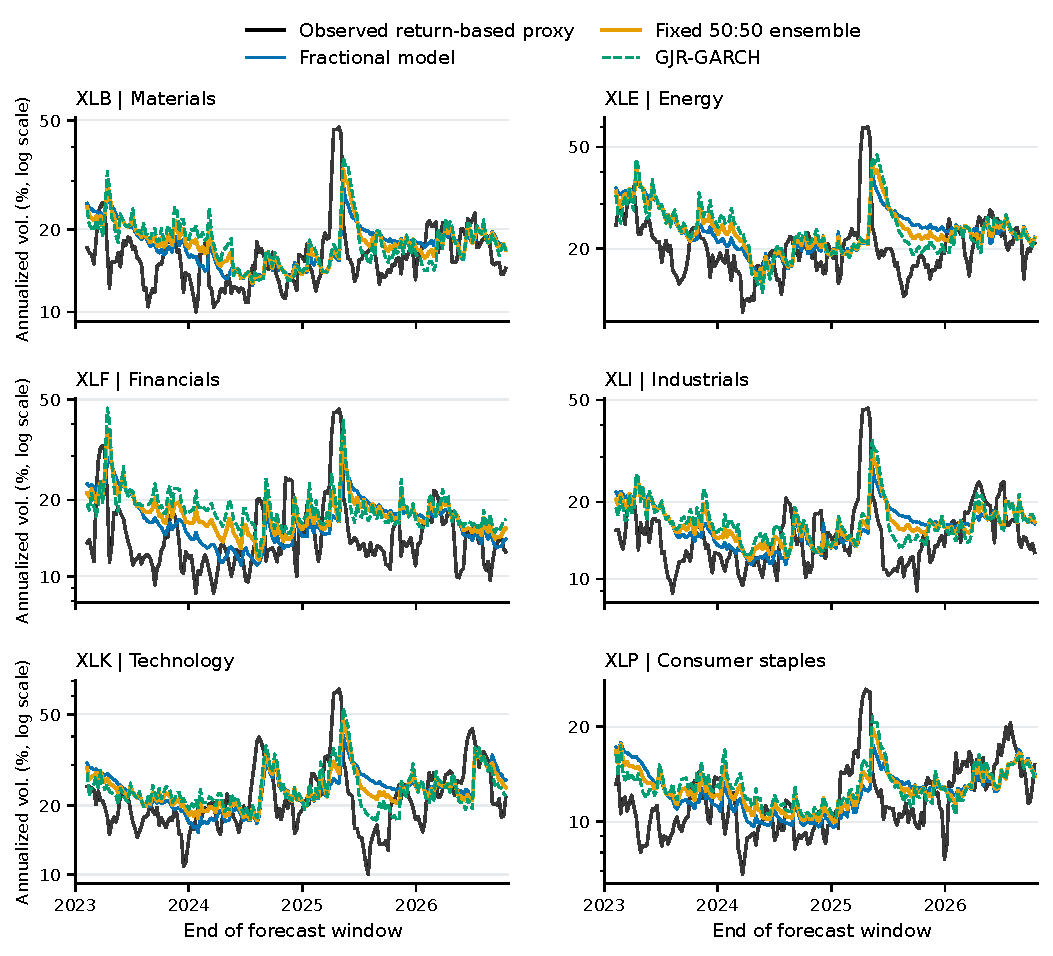
\includegraphics[width=\textwidth,height=.70\textheight,keepaspectratio]{figures/prediction_sectors_a.pdf}
\caption{Twenty-one-session observed proxies and forecasts for materials,
energy, financials, industrials, technology and consumer staples. Curves use
the same methods and colors as Figure~\ref{fig:index-predictions}.}
\label{fig:sectors-paths-a}
\end{figure}

\begin{figure}[p]
\centering
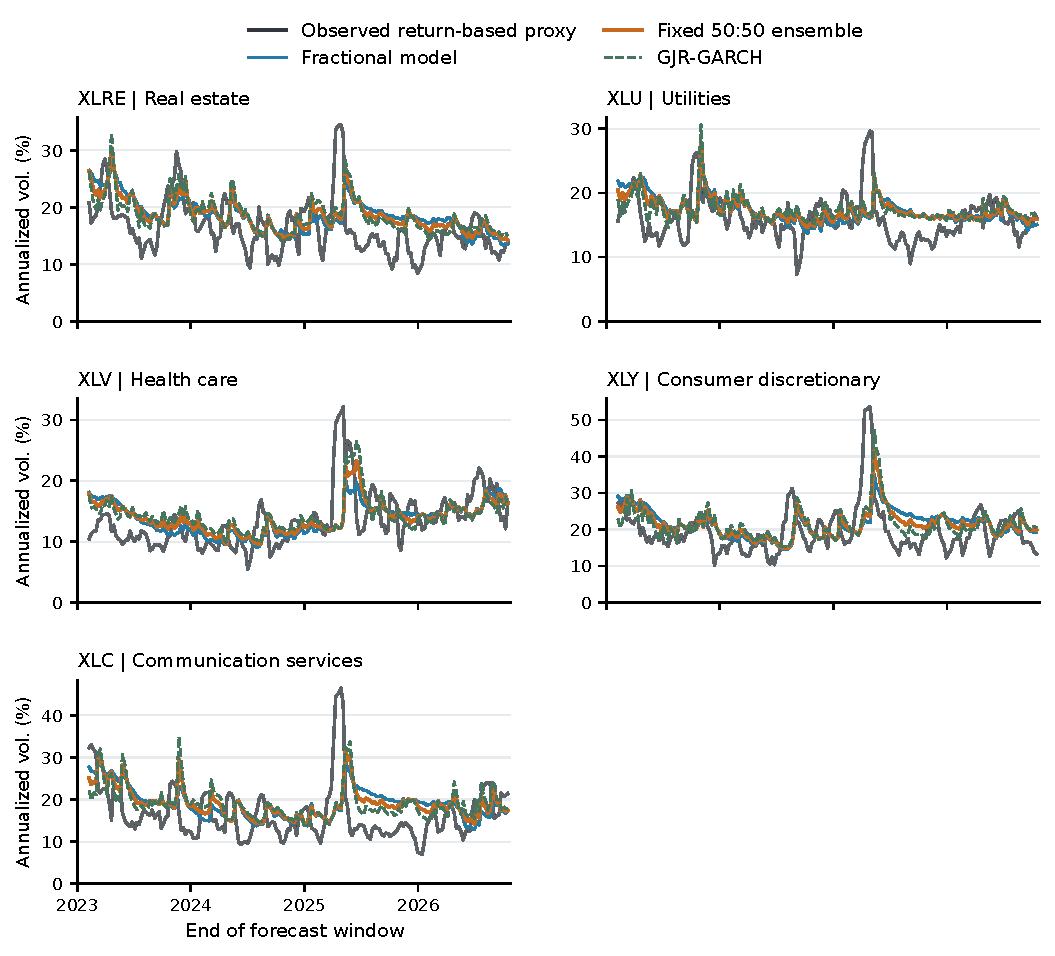
\includegraphics[width=\textwidth,height=.78\textheight,keepaspectratio]{figures/prediction_sectors_b.pdf}
\caption{The remaining five sector ETFs: real estate, utilities, health care,
consumer discretionary and communication services. Every sector is included
exactly once across these two figures.}
\label{fig:sectors-paths-b}
\end{figure}

\begin{figure}[p]
\centering
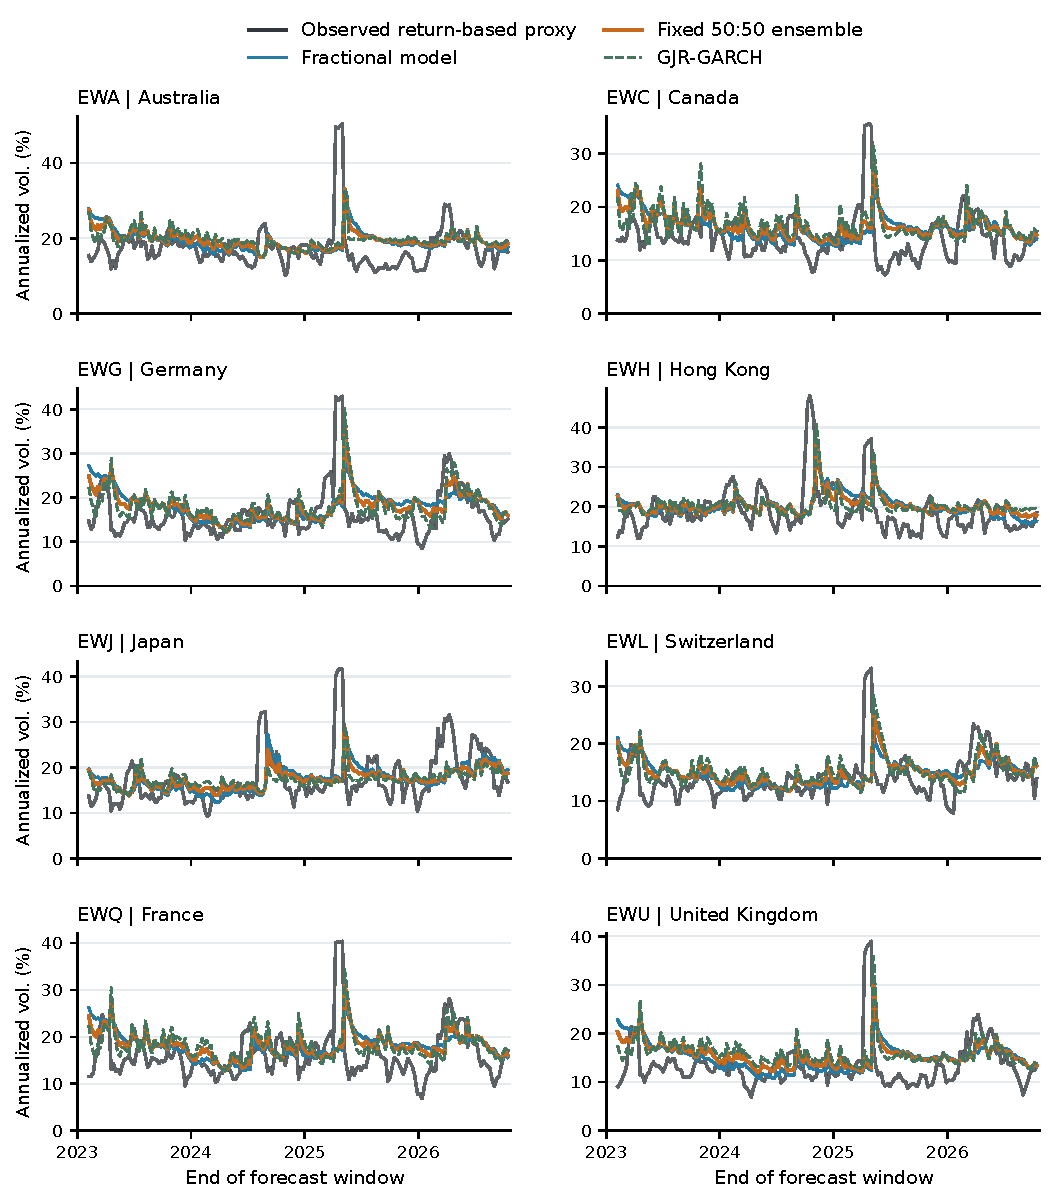
\includegraphics[width=\textwidth,height=.80\textheight,keepaspectratio]{figures/prediction_countries.pdf}
\caption{Twenty-one-session observed proxies and forecasts for all eight
pre-specified country ETFs. The observed series is a noisy daily-return-based
proxy; the plots do not imply prediction of the underlying ETF price direction.}
\label{fig:countries-paths}
\end{figure}

\clearpage
\bibliographystyle{unsrtnat}
\bibliography{references}
\end{document}
